\documentclass{article}
\usepackage[utf8]{inputenc}
\usepackage[a4paper, portrait, margin=1in]{geometry}
\usepackage{graphicx}
\usepackage{subcaption}
\usepackage{tabularx}
\usepackage{hyperref}
\hypersetup{
    colorlinks=true,
    linkcolor=blue,
    filecolor=magenta,      
    urlcolor=cyan,
}
\usepackage{amsmath}

\title{Cloud Computing (UE18CS352) \\Unit 5}
\author{Aronya Baksy}
\date{April 2021}

\begin{document}

\maketitle
\section{Proxies in the cloud}
\subsection{Reverse Proxy}
\begin{itemize}
    \item A reverse proxy receives HTTP connection requests from clients and routes the traffic to the application's origin server. Reverse proxies are maintained by the owner of the origin server.
    
    \item Reverse proxy servers (implemented in Apache, Nginx, Caddy) can inspect HTTP headers and route requests directed at a single IP address to any one of many internal servers based on the domain name. 
    
    \item Reverse proxy servers improve security, performance and reliability
    
    \item Operation:
    \begin{enumerate}
        \item Receive connection request from client 
        
        \item Complete the three-way TCP handshake, terminate the orignal connection, connect with the origin server and complete the request.
    \end{enumerate}
    
    \item Benefits:
    \begin{itemize}
        \item Application security
        
        \item Load balancing when the origin server is replicated across multiple machines
        
        \item Caching
        
        \item SSL encryption
    \end{itemize}
\end{itemize}
\begin{figure}[!h]
    \centering
    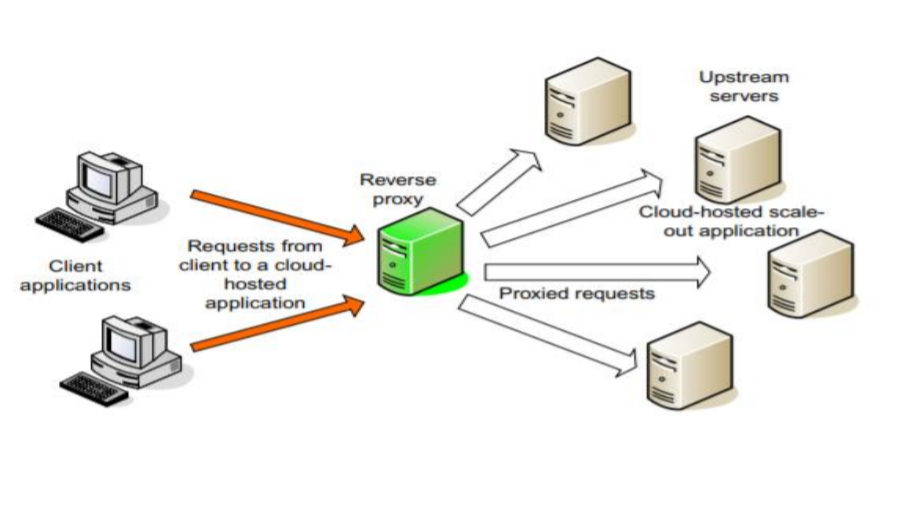
\includegraphics[scale=0.65]{p1.png}
    \caption{Reverse Proxy Configuration}
    \label{fig:my_label}
\end{figure}
\subsection{Forward Proxy}
\begin{itemize}
    \item Regulates outbound traffic in accordance with certain policies in shared networks. Collects requests from clients, and interacts with servers on behalf of the client. 
    
    \item Forward proxies are useful in order to :
    \begin{itemize}
        \item Block access to certain websites for an organization, and monitor organization's online activities. 
        
        \item Block malicious traffic from reaching origin servers. 
        
        \item Cache external site content and hence reduce response times. 
    \end{itemize}
\end{itemize}

\subsection{Nginx}
\begin{itemize}
    \item Nginx is a web server that can also be used as a reverse proxy, load balancer and HTTP cache. 
    
    \item Load balancing is either done using round-robin scheduling, or the optional hash-based scheduler that chooses an upstream server based on the hash of some value (can be request URL, incoming HTTP headers, or some combination of the same)
    
    \item Scaling is done by simply changing the Nginx server configuration i.e. by adding more servers and the corresponding IP addresses in the "upstream" section
\end{itemize}

\section{Scalability}
\begin{itemize}
    \item Ability to increase/decrease IT resources deployed in response to changing workloads and demands. 
    
    \item Scaling can be done for data storage, compute or networking, and must be done with minimal downtime or service disruption. 
    
    \item Elasticity refers to the system's ability to allocate or deallocate resources for itself in response to changing workloads
    
    \item On the other hand, scalability refers to the ability to use only existing resources to handle increased workloads
    
    \item The tradeoff between Elasticity and scalability depends on the app's workloads being predictable or highly variable.
\end{itemize}
\subsection{Benefits of cloud scalability}
\begin{itemize}
    \item \textbf{Cost Saving}: pay-as-you-go model, avoid purchasing expensive hardware that soon may become obsolete
    
    \item \textbf{Disaster Recovery} costs are reduced as need for maintaining secondary data centers is eliminated
    
    \item \textbf{Convenience}: rapid provisioning of resources, customized to organization needs
    
    \item \textbf{Flexibility} in handling variable workloads with minimal costs, helps small businesses greatly. 
\end{itemize}

\subsection{Scaling Strategies}
\subsubsection{Vertical Scaling}
\begin{itemize}
    \item Adding more resources (CPU, Memory, Disk, I/O) to an existing server, or replacing an existing server with a more powerful one. 
    
    \item AWS and Azure support vertical scaling by changing instance types. 
    
    \item AWS and Azure cloud services have many different instance sizes, so scaling vertically is possible for many types of resources (EC2 instances, RDS databases)
\end{itemize}
\subsubsection{Horizontal Scaling}
\begin{itemize}
    \item Adding more instances of the same existing configuration and splitting workloads between the new increased number of instances
    
    \item Increase number of instances instead of changing instance type
\end{itemize}
Think of it like this, vertical scaling is adding more floors to a single house, whereas horizontal scaling is building 2 more houses of the same size as the existing one. 

\subsection{Scaling through Reverse Proxies}
\begin{itemize}
    \item The reverse proxy might even be configured as a load balancer.
    
    \item To the outside world there is just a single server, but the load balancer takes each request and forwards it on to an application server on the private network.
    
    \item Load balancer decides which server should receive the request based on some scheduling algorithm. 
\end{itemize}

\section{Hybrid Cloud and Cloud Bursting}
\begin{itemize}
    \item Combination of private and public clouds enabling expansion of local infrastructure to commercial infrastructure on a need basis
    
    \item Organizations can leverage existing infrastructure and supplement it with cloud resources as per demand
    
    \item \textbf{Cloud bursting} is an configuration between public and private clouds that allows for uninterrupted service by sending excess traffic beyound the capability of the private cloud, to the public cloud. 
    
    \item Hybrid cloud enables Cloud Bursting of the private cloud by allowing the addition of extra capacity to a private infrastructure by borrowing from a public cloud
    
    \item Benefits of cloud bursting
    \begin{itemize}
        \item Flexible and cost-effective solution to manage sudden workloads seamlessely.
        
        \item Simple to manage scaling up/down of resources in public cloud
        
        \item Cost savings on internal hardware procurement for an organization. Internal Compute resources Freed up for better usage in other areas.
        
        \item Improved customer experience and customer retention levels due to uninterrupted access to the application.
    \end{itemize}
\end{itemize}

\section{Multi-Tenancy}
\begin{itemize}
    \item An architecture model wherein a single instance of an application or a hardware serves multiple clients. 
    
    \item Three types of multi-tenancy models:
    \begin{itemize}
        \item Shared Machine: each client has their own DB process and tables on a single shared machine
        
        \item Shared-Process: Each client has their own tables, but only one database process executes queries for all clients
        
        \item Shared-Table: clients share database tables and process. 
    \end{itemize}
\end{itemize}

\subsection{Requirements of a Multi-Tenant System}
\begin{itemize}
    \item Fine-grained resource sharing: leads to greater scalability, but also necessitates better access control and security.
    
    \item Security and isolation between tenants
    
    \item Customization of tables
\end{itemize}

\subsection{Types of Multi-tenant Architectures}
\subsubsection{Single multi-tenant database}
\begin{itemize}
    \item A single app instance, and a single database instance. 
    
    \item Highly scalable. As more tenants are added, the database is scaled up by adding more storage.
    
    \item Low cost due to shared resources, but high operational complexity during design and setup
\end{itemize}

\subsubsection{One Database per Tenant}
\begin{itemize}
    \item Single app instance, one DB instance per tenant. 
    
    \item Higher cost and less scalable than single multi-tenant architecture, but operational complexity is low.
    
    \item Scalability may be achieved by adding more DB nodes.
\end{itemize}

\subsubsection{Single-Tenant App with Single-Tenant DB}
\begin{itemize}
    \item The entire app is installed separately for each tenant. Each tenant has their own app instance and their own DB instance. 
    
    \item Highest level of data isolation, but high cost due to extra hardware needed to support.
\end{itemize}

\subsection{Levels of Multi-Tenancy}
\subsubsection{Ad-Hoc or Custom Instances}
\begin{itemize}
    \item Each tenant has their own custom version of software. 
    
    \item Found in current enterprise data centers. 
    
    \item Management is difficult as each customer needs specialized management support.
\end{itemize}

\subsubsection{Configurable Instances}
\begin{itemize}
    \item All tenants share same version of program, but configuration is possible to an extent. 
    
    \item Significant management savings as only one copy of the software is to be maintained.
\end{itemize}

\subsubsection{Configurable, Multi-Tenant instances}
\begin{itemize}
    \item Only one instance of the running program is shared by all customers.
    
    \item Leads to additional efficiency in resource usage as well as management
\end{itemize}

\subsubsection{Scalable, configurable multi-tenant instances}
\begin{itemize}
    \item Instances can scale up or down depending on the number of customers, and demand of each customer.
    
    \item Peformance bottlenecks and capacity limitations from other levels are eliminated here to an extent
\end{itemize}

\subsection{Challenges of Multi-Tenancy}
\subsubsection{Authentication}
\begin{itemize}
    \item Secure sharing of resources is enforced using authentication
    
    \item In a \textit{centralized authentication system}, auth takes place using a centralized user database. The cloud admin gives the tenants the right to manage their own accounts on this database. 
    
    \item In a \textit{decentralized authentication system}, each tenant maintains their own user database, and the tenant deploys a federation service that interfaces between the authentication services of tenant and cloud.
\end{itemize}

\subsubsection{Implementing Resource Sharing}
\begin{itemize}
    \item Access control is provided using \textbf{roles} and \textbf{business rules}. 
    
    \item A \textit{role} is associated with a set of permissions specific to it. The ability to set permissions for roles is also attached to a certain small set of roles. 
    
    \item A \textit{business rule} is a policy that provides fine-grained access control, based on the context of the running application (e.g. in a banking app, limit the amt of money withdrawn in a single transaction, or limit the time during which transaction can take place)
    
    \item Business rules are implemented using policy engines like Drools Guvnor and Drools Expert
    
    \item Two types of access control:
    \begin{itemize}
        \item \textbf{Access Control List}: Each object associated with a set of permissions for each role
        
        \item \textbf{Capability-based Access Control}: If a user holds a reference or capability (called a \textbf{key}) to an object, they have access to the object. 
    \end{itemize} 
\end{itemize}

\subsubsection{Sharing Storage Resources}
\begin{itemize}
    \item In a \textbf{shared table} approach, all tenant's data is stored in a single table. A \textit{metadata table} stores info about tenants.
    
    \item Shared table is more space efficient but requires multiple select statements for a query (to join between metadata table and actual data table)
    
    \item In a \textbf{dedicated table} approach, each tenant has their own table. Access to other tenant's tables is restricted. 
\end{itemize}

\section{Cloud Security}
\begin{itemize}
    \item A set of control-based safeguards and technologies that protect cloud resources from online theft, leakage or data loss. 
    
    \item Cloud security is partitioned into the physical and virtual domains. Basic objectives of cloud security are confidentiality, integrity and availability
\end{itemize}

\subsection{Physical Security}
\begin{itemize}
    \item Physical security involves protection against physical threats like intruders, natural disasters and human error (e.g. forgot to turn on the AC)
    
    \item Multi-layered physical security system involves:
    \begin{enumerate}
        \item Central monitoring and control center with dedicated staff
        
        \item Monitoring for each type of physical threat
        
        \item Training of staff in response to threat situations
        
        \item Manual or automated backup systems to mitigate damage caused
        
        \item Secure access to facility
    \end{enumerate}
\end{itemize}

\subsection{Virtual Security: Best practices}
\subsubsection{Cloud Time Service}
\begin{itemize}
    \item Synchronize all nodes in the data center to the same clock. 
    
    \item Synchronization is needed for correct ordering of operations, as well as analysis of system logs across geographically distributed locations
    
    \item Network Time Protocol (NTP) is used for this. Encryption is used to avoid fake reference sources. 
\end{itemize}

\subsubsection{Identity and Access Management}
\begin{itemize}
    \item IM must be scalable, federated, allow single identity and single sign-in and must satisfy legal and policy requirements. 
    
    \item Access Management allows access to cloud facilities only to authorized users. 
    
    \item In addition, it controls the access of cloud management personnel, implements 2-factor authentication, disallows shared accounts and white lists IP addresses to allow remote access. 
\end{itemize}

\subsubsection{Break-glass protocols}
\begin{itemize}
    \item In case of emergencies, bypass normal security controls and allow an alarm to be triggered
    
    \item Such a protocol must ensure that it can be executed only in emergencies under controlled situations and that the alarm is triggered properly. 
\end{itemize}

\subsubsection{Key Management}
\begin{itemize}
    \item Secure facilities for the generation, assignment, revocation, and archiving of keys. 
    
    \item Also generate procedures for recovering from compromised keys
\end{itemize}

\subsubsection{Auditing}
\begin{itemize}
    \item Capture all security-related events, together with data needed to analyze the event 
    
    \item This data includes time, system on which the event occurred, and userid that initiated the event. 
    
    \item The audit log is centralized and secure
    
    \item It must be possible to create a sanitized or stripped-down version to share with cloud customers for further analysis. 
\end{itemize}

\subsubsection{Security Monitoring and Testing}
\begin{itemize}
    \item Monitoring involves a system-wide anomaly and intrusion detection system installed on network and host nodes. 
    
    \item At times, cloud users can create their own anomaly and intrusion detection systems.
    
    \item All software (releases or patches) are tested in a test bed environment before deployment to production environment.
    
    \item Testing happens on a continuous ongoing basis that identifies vulnerabilities in the cloud system. 
\end{itemize}

\subsection{Risk Management in Cloud}
\begin{itemize}
    \item Risks in data security and resource outages can be crippling for dependent organizations.
    
    \item Risk management is the process of identifying, evaluating, monitoring and controlling risks in a business environment.
    
    \item Risk management is domain dependent, and must tradeoff between risk impact and cost of risk mitigation measure.
    
    \item A \textbf{security control} is a safeguard that detects, responds or prevents a security risk. There are three broad categories of security controls: technical, operational and Management, with each further divided into 18 families.
    
    \item Security breaches are classified as low-impact, medium-impact or high-impact based on the requirement for security control. 
    
    \item \textbf{Low Impact Systems} are those where a security breach causes \textit{limited degradation in capability}, but the system can still perform its primary functions.
    
    \item \textbf{Medium Impact Systems} are those where the system is still capable of performing its primary functions but there is a \textit{significant degradation in the capabilities}.
    
    \item \textbf{High-Impact Systems} are those where a security breach causes \textit{inability to perform primary functions}. 
\end{itemize}
\subsubsection{Risk Management Process}
\begin{itemize}
    \item Categorize information resources on the basis of criticality (impact in case of failure) and sensitivity (confidentiality)
    
    \item Select security controls appropriate to the levels of criticality and sensitivity chosen
    
    \item Evaluate the chosen security controls. Upgrade them if found insufficient against anticipated threats.
    
    \item Implement chosen security controls. These may be administrative, technical or physical. 
    
    \item Monitor effectiveness of deployed security controls
    
    \item Periodic review of all security controls must take place to protect against new threats, and to account for operational changes in system design etc. 
\end{itemize}

\subsection{Security Design Patterns}
\subsubsection{Defense in Depth}
\begin{itemize}
    \item Layered defenses protect sensitive resources. 
    
    \item e.g.: Remote access to a cloud allowed only through VPN. Access could be allowed only from certain whitelisted IP addresses. Admins may be needed to further provide a OTP for access. 
\end{itemize}

\subsubsection{Honeypot}
\begin{itemize}
    \item Honeypots are systems that disguise themselves as valuable targets, while being monitored by security personnel.
    
    \item While an attacker attempts to control the honeypot, the sysadmins monitoring the honeypot can trap and stop the attack. 
    
    \item Honeypot VMs can be deployed by the cloud provider or the cloud customers.
\end{itemize}

\subsubsection{Sandboxing}
\begin{itemize}
    \item Execution of software inside a controlled environment within an operating system.
    
    \item Within the sandbox, the software has access only to the bare minimum resources it needs to function properly. Hence any attacker gaining control of the software does not have unrestricted access to the entire system.
    
    \item Sandboxes also provide defense in depth as any attacker is also needed to overcome the sandbox in order to gain unrestricted access. 
\end{itemize}

\subsection{Network Design Patterns for Security}
\subsubsection{VM Isolation}
\begin{itemize}
    \item Encryption of traffic between VMs, or tightened network controls on VMs (using ACLs, restricting port numbers)
\end{itemize}

\subsubsection{Subnet Isolation}
\begin{itemize}
    \item Separate subnets for admin traffic, user traffic and storage network traffic.
    
    \item Physically separate networks are preferred as virtual LANs (VLAN) that are not physically separate are hard to configure correctly.
    
    \item Routing between the networks is handled by firewalls.
\end{itemize}

\subsubsection{Common Management DB}
\begin{itemize}
    \item a database that contains information regarding the components of an IT system (inventory of components, present config and status)
    
    \item Simplifies implementation and management of IT services, allows all admins to have a consistent view of the IT system. 
\end{itemize}

\subsection{Example of PaaS Security}

\begin{figure}[!h]
    \centering
    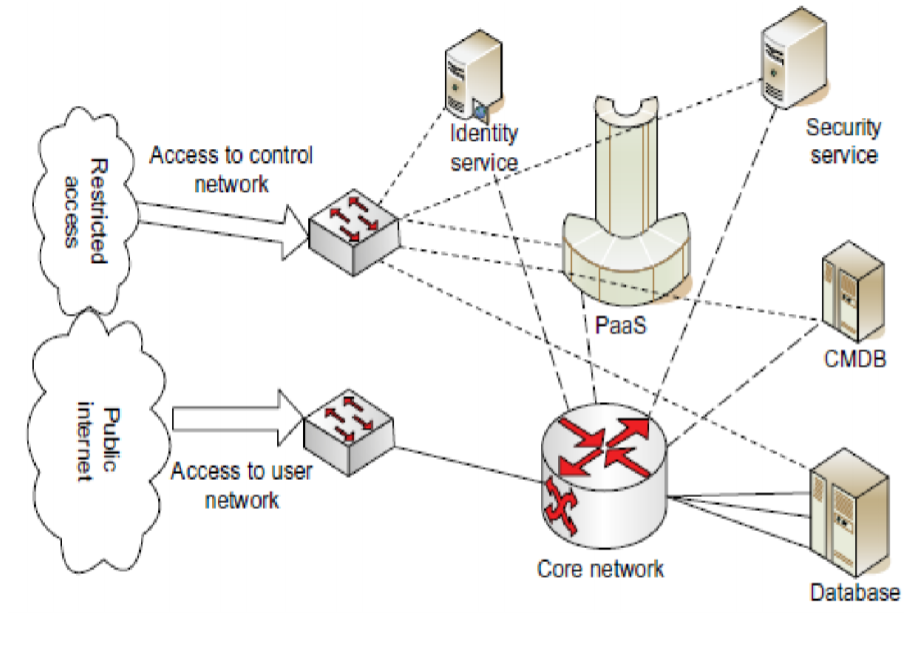
\includegraphics[scale=0.7]{p2.png}
    \caption{Security Architecture for PaaS System}
    \label{fig:my_label_2}
\end{figure}

\subsubsection{External Network Access}
\begin{itemize}
    \item Distinct interfaces for distinct physical networks, one for admins and one for cloud users. 
    
    \item Access to control network is limited to whitelisted IP addresses only. 
    
    \item Multi-factor authentication can be made mandatory for increasing secure access to administrative functions. 
    
    \item The access to the public network is via two switches, to increase availability via redundancy.
\end{itemize}

\subsubsection{Internal Network Access}
\begin{itemize}
    \item Separate physical networks for admin control functions and one for cloud user functions. Protects control network from unauthorized access.
    
    \item The DBMS is connected to the public network via an aggregated set of links to provide increased bandwidth and availability.
    
    \item PaaS service is accessible from public and private networks. But the security server need not be accessible from the public network.
\end{itemize}

\subsubsection{Database Server Security}
\begin{itemize}
    \item The identity server handles access management to the database. 
    
    \item Database is further secured by restricting the allowed ports on which internet traffic is allowed. 
    
    \item Additional security is implemented by checking the validity of the ODBC connection from the client to the database
\end{itemize}

\subsubsection{Security Service}
\begin{itemize}
    \item The diagram also includes a security server to perform security services such as
    
    \begin{itemize}
        \item Auditing of security
        
        \item Monitoring for security threats
        
        \item Hosting a security operations center
        
        \item Security scanning of the cloud infrastructure
    \end{itemize} 
\end{itemize}

\subsection{Standards for Security Architecture}
\subsubsection{SSE-CMM}
\begin{itemize}
    \item System Security Engineering Capability Maturity Model, adaptation of CMM for software projects by CMU
    
    \item Defines 5 capability levels for an organization
    
    \item Allows organizations to plan and implement processes for self improvement
\end{itemize}

\subsubsection{ISO/IEC 27001-27006}
\begin{itemize}
    \item Set of related standards under the ISO/IEC 27000 family that provides an Info. Security Management System. 
    
    \item Specifies requirements to be satisfied by all organizations, and processes for evaluating security risks
    
    \item Not specific to cloud
\end{itemize}

\subsubsection{ENISA}
\begin{itemize}
    \item European Network and Info. Security Agency provides a \textbf{Cloud Computing Information Assurance Framework}. 
    
    \item The framework is a set of assurance criteria designed to assess the risk of adopting cloud services, compare different Cloud Provider offers, obtain assurance from the selected cloud providers, and reduce the assurance burden on cloud providers
\end{itemize}

\subsubsection{ITIL Security Management}
\begin{itemize}
    \item ITIL is a comprehensive set of standards used for ITSM, based on ISO/IEC 27002. 
    
    \item Shallow learning curve due to the fact that ITIL  is already adopted in many data centers. 
\end{itemize}

\subsubsection{COBIT}
\begin{itemize}
    \item Control OBjectives for Information related Technologies, developed by the ISACA.
    
    \item A set of best practices for linking business and IT goals, with metrics and maturity models. 
    
    \item Broader scope than ISO/IEC 27000
\end{itemize}

\subsubsection{US NIST}
\begin{itemize}
    \item US National Institute for Standards and Technology releases many whitepapers in the Security Management and Assurance working group. 
    
    \item Targeted at US Federal Agencies (CIA, FBI etc.) , but apply to many organizations as well. 
\end{itemize}

\subsection{Legal and Regulatory Issues with the cloud}
\begin{itemize}
    \item Local, national and international laws apply due to distributed nature of the cloud, as well as the presence of a third party (i.e. the cloud provider)
    
    \item Such laws must specify who is responsible for security and accuracy of the data stored on cloud. 
    
    \item Issues to consider when framing laws:
    \begin{itemize}
        \item Cover all risks arising from a third party's presence 
        
        \item Need to ensure data security 
        
        \item Obligations of the cloud provider during any litigation
    \end{itemize}
\end{itemize}
\subsection{Legal Issues}
\subsubsection{Due Diligence}
\begin{itemize}
    \item Client must define scope of service provided, as well as regulations and compliance standards to be followed
    
    \item Consider any risks arising from stability and reliability of the cloud provider, as well as the criticality of the business function outsourced to the cloud.
\end{itemize}

\subsubsection{Contract Negotiation}
\begin{itemize}
    \item Cloud services may have one-click standard agreements that are not customizable. Such agreements are acceptable for low-risk scenarios.
    
    \item Cloud service providers can avoid negotiating custom agreements with each customer through external accreditations
\end{itemize}

\subsubsection{Implementation}
\begin{itemize}
    \item Enterprise must ensure that the safeguards laid out in the contract are actually being followed
    
    \item It is also important to continuously re-evaluate the system periodically to check for changed circumstances (increased data sensitivity, revoked external certifications)
\end{itemize}

\subsubsection{Contract Termination}
\begin{itemize}
    \item Identify alternate service provider, ensure timely and secure transfer of services
    
    \item Also ensure that sensitive data if any, is completely deleted from the original provider's systems.
\end{itemize}

\subsubsection{Data Privacy and Secondary use of Data}
\begin{itemize}
    \item Use collected data only for intended purpose, and such data cannot be sold to third parties 
    
    \item Privacy laws often state that individuals can access their own data and modify or delete it
    
    \item Enterprises must ensure that cloud service providers do not use the data for
data mining or other secondary usage.

\end{itemize}

\subsubsection{Data Location}
\begin{itemize}
    \item Data handling laws differ between countries, hence transferring data between countries is a challenging process. 
    
    \item Allow for the location of data to be known in advance so that such scenarios can be planned (e.g. AWS allows selection of regions for all services)
    
    \item The enterprise must obey the most stringent of all the laws that apply across the countries where data is stored. 
\end{itemize}

\subsubsection{Business Continuity Planning}
\begin{itemize}
    \item BCP is used to implement actions to keep a business running in the face of natural disasters that affect infrastructure, including those maintained on a third-party cloud. 
    
    \item BCP typically involves identifying the possible catastrophes, carrying out Business Impact Analysis, and using the results of the analysis to formulate a recovery plan
    
    \item Disaster Recovery planning (DRP) is a part of BCP used for recovery of IT operations. 
    
    \item BCP and DRP are made before deploying apps to cloud, and implemented during the deployment. Some cloud providers provide features (e.g. multi-locations) that help in BCP and DRP
\end{itemize}

\subsubsection{Security Breaches}
\begin{itemize}
    \item In case of a breach, cloud provider's disclosure policy is important. 
    
    \item Disclosure policy defines how quickly a customer is notified of a breach, so that corrective action can be taken. 
    
    \item To avoid ambiguity, the service agreement should specify the actions to be taken during a breach
\end{itemize}

\subsubsection{Litigations}
\begin{itemize}
    \item During a litigation against an enterprise or a cloud provider, the provider must be able to make available any data that is needed for this litigation. 
    
    \item This is important as enterprises (not cloud providers) are responsible for responding to such requests. 
    
    \item In case a cloud provider is directly requested to provide data, then the affected business must be contacted and must be given the opportunity to oppose the request. 
\end{itemize}

\section{Cloud Authentication: Keystone}
\begin{itemize}
    \item Keystone is an OpenStack service that provides:
    \begin{itemize}
        \item API client authentication
        
        \item Service discovery
        
        \item Ditributed multi-tenant authorization
    \end{itemize}
    using OpenStack's Identity API
    
    \item The fundamental purpose of Keystone is to be a registry of projects and decide on access to projects. 
\end{itemize}

\subsection{Terminologies}
\subsubsection{Project}
\begin{itemize}
    \item An abstraction used to group resources (servers, machine images etc.)
    
    \item Users or user groups are given access to projects using role assignments. 
    
    \item The specific role assigned outlines the type of access and capabilites that a user/user group is entitled to.
\end{itemize}

\subsubsection{Domain}
\begin{itemize}
    \item AN abstraction that isolates the visibility of a set of projects and users (or user groups) to a single organization
    
    \item Domains enable splitting cloud resources into silos that can be used by each organization. 
    
    \item Domains represents logical divisions within an enterprise, or maybe entirely different enterprises
\end{itemize}

\subsubsection{Users and User Groups}
\begin{itemize}
    \item Also known as actors, they are the ones who utilize the cloud resources. 
    
    \item User groups are groups of users that have some shared responsibility. 
\end{itemize}

\subsubsection{Relationship between the three}
Domains are a collection of Users, Groups, and Projects. Roles are globally
unique. Users may have membership in many Groups.

\subsubsection{Roles}
\begin{itemize}
    \item "Assigned to" an user and "assigned on" a project. 
    
    \item Convey a sense of authority, a particular responsibility to be fulfilled by an actor. 
    
    \item A role assignment is a triple of actor, target (may be a project or a domain), and a role.
    
    \item Role assignments can be granted, revoked and inherited between users/projects. 
\end{itemize}

\subsubsection{Token}
\begin{itemize}
    \item Each API call authenticated by Keystone requires the passing of a token. 
    
    \item Tokens are generated by Keystone upon successful authentication of an user against the service. 
    
    \item A token has both an unique ID (unique per cloud) and a payload (data about the user)
\end{itemize}

\subsubsection{Service Catalog}
\begin{itemize}
    \item List of endpoints and URLs for different services on a cloud. 
    
    \item Used mainly for service discovery and access (such as creating VMs, storage allocation etc.)
    
    \item Each endpoint is broken down into a public URL, an internal URL and an admin URL (all may be the same or not)
\end{itemize}

\subsection{Identity in Keystone}
\subsubsection{SQL}
\begin{itemize}
    \item Identity of actors (name, password, metadata) and groups stored on an SQL database (MySQL, PostgreSQL, DB2) 
    
    \item Keystone in this case serves as the identity provider
    
    \item Pros:
    \begin{itemize}
        \item Easy setup
        
        \item Manage users and groups via OpenStack APIs
    \end{itemize}
    
    \item Cons:
    \begin{itemize}
        \item Keystone should not be identity provider as well as authenticator
        
        \item Weak password support: no password rotation or recovery
        
        \item Does not integrate with existing enterprise LDAP servers
    \end{itemize}
\end{itemize}

\subsubsection{LDAP}
\begin{itemize}
    \item Keystone can retrieve and store actors (Users and Groups) in Lightweight Directory Access Protocol (LDAP).
    
    \item LDAP should be restricted to only read operations (searching) and authentication (bind). 
    
    \item Keystone needs a minimal amount of privilege to use the LDAP (read access to attrs defined in the configuration, as well as an anonymous access)
    
    \item Pros:
    \begin{itemize}
        \item No need to maintain copies of user accounts
        
        \item Keystone no longer acts as identity provider
    \end{itemize}
    
    \item Cons:
    \begin{itemize}
        \item Service accounts need to be stored somewhere (may not be desirable to have them on LDAP server)
        
        \item Keystone is still seeing user passwords in the request messages. Ideally Keystone should never see user passwords. 
    \end{itemize}
\end{itemize}

\subsubsection{Multiple backends}
\begin{itemize}
    \item Allow one identity source per Keystone domain. 
    
    \item Allows service accounts and employee accounts to be separated, and allows use of multiple LDAPs for flexibility in organization of departments.
    
    \item Pros:
    \begin{itemize}
        \item Support multiple LDAPs for various user accounts, SQL for service accounts
        
        \item Leverage existing LDAP identity
    \end{itemize}
    
    \item Cons:
    \begin{itemize}
        \item Complex set up
        
        \item User authentication must be domain-scoped
    \end{itemize}
\end{itemize}

\subsubsection{Identity Providers}
\begin{itemize}
    \item An identity provider is a service that abstracts the identity service backed and translates user information into some standard federated identity protocol.
    
    \item Keystone uses Apache modules for consuming authentication info from multiple Identity Providers. 
    
    \item Such users never stored in Keystone, not permanent, users will have their attributes mapped into group-based role assignments
    
    \item From a Keystone perspective, an identity provider is a source for identities; it may refer to software that is backed by various backends or Social Logins
    
    \item Pros:
    \begin{itemize}
        \item Leverage existing infra \& software for user authentication
        
        \item Separation between Keystone service and user info
        
        \item Keystone never sees any user passwords
        
        \item Type of authentication (certificate-based, 2-factor) is abstracted away from keystone
    \end{itemize}
    
    \item Con: most complex setup
\end{itemize}

\subsection{Authentication in Keystone}
\subsubsection{Password}
\begin{itemize}
    \item User or service provides a password for authentication
    
    \item The payload of the request contains information needed to find where the user exists, authenticate the user, and optionally, retrieve a service catalog based on the user’s permissions on a scope
    
    \item The user section identifies the user (either on a domain, or using a globally unique user ID), 
    
    \item The scope section identifies the project being worked on, and hence is used to retrieve the service catalog. Must contain information to identify a project and the owning domain. 
\end{itemize}

\subsubsection{Token}
\begin{itemize}
    \item A user may also request a new token by providing a current token.
    
    \item The payload contains the current token ID. 
    
    \item This allows refreshing a token that will soon expire, or changing a token type from unscoped to scoped. 
\end{itemize}

\subsubsection{Access Management}
\begin{itemize}
    \item Keystone manages access to APIs using \textbf{role-based access control}.  
    
    \item Consists of policies stored in JSON form at each API endpoint. 
    
    \item Rules in JSON form consists of target:rule pairs. 
    
    \item At the top of the file, targets are established that can be used for evaluation of other targets. 
    
    \item Here the meaning of admin, owner and other roles are defined.
\end{itemize}
\begin{figure}[!ht]
    \centering
    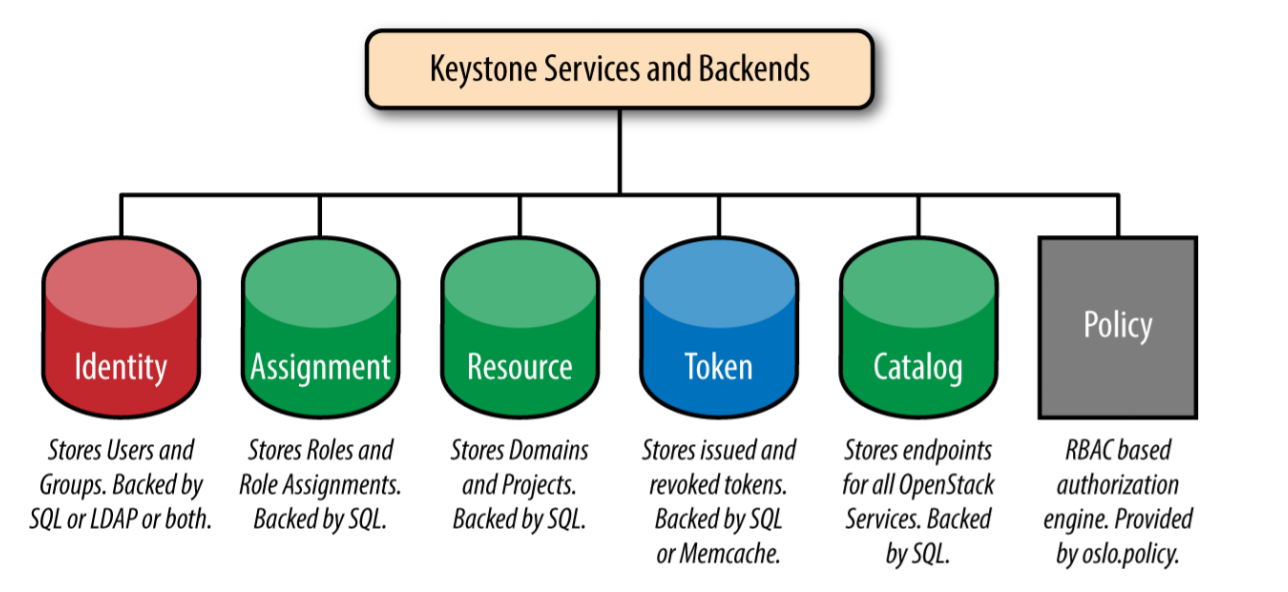
\includegraphics[scale=0.5]{p3.png}
    \caption{Keystone Services and Backends}
    \label{fig:my_label_3}
\end{figure}

\section{Cloud Security Threats: Denial of Service}
\begin{itemize}
    \item A type of cyber attack in which a malicious actors aim to render a device unavailable to its intended users by interrupting the device's normal functioning. 
    
    \item DoS attacks typically function by overwhelming or flooding a targeted machine with requests until normal traffic is unable to be processed, resulting in denial-of-service to addition users.
    
    \item The focus of a DoS attack is to overpower the capacity of a targeted machine, resulting in denial-of-service to additional requests.
    
    \item Types of DoS attacks
    \begin{itemize}
        \item \textbf{Buffer Overflow}: force a machine to consume resources until capacity runs out. Leads to slow response time, system crashes and hence DoS
        
        \item \textbf{Flood Attacks}: Overpower the server by targeting a server with a massive number of packets. For this attack the attacker must have greater bandwidth than the target. 
    \end{itemize}
\end{itemize}

\subsection{DDoS Attacks}
\begin{itemize}
    \item \textbf{Distributed DoS (aka DDoS) attacks} utilize multiple computers as sources of attack traffic.
    
    \item DDoS attacks are carried out with networks of internet-connected machines that have been infected with a malware that allows an attacker to control them remotely. 
    
    \item Such a network of machines is called a botnet (with individual machines being called bots or zombies). Each bot is a legitimate machine on the internet hence it is difficult to separate attack traffic from actual traffic. 
    
    \item The botnet floods the victim with requests, overwhelming the capacity and causing denial of service. 
\end{itemize}

\subsection{EDoS: Economic Denial of Sustainability}
\begin{itemize}
    \item EDoS targets the vulnerabilities of cloud computing's utility pricing model. 
    
    \item EDoS attackers steadily send illegitimate traffic to gradually consume cloud resources such as VMs, network devices, security devices and DBs so that it can trigger auto scaling features of cloud
    
    \item Consequently, due to the additional resource usage, the target consumer is billed for additional charges, causing financial problems.
    
    \item The other side effect of this attack is the persistent degradation of services faced by benign cloud users.
\end{itemize}

\begin{tabular}{|p{0,45\textwidth}|p{0.45\textwidth}|}
    \hline
    \textbf{DDoS Attack} & \textbf{EDoS Attack} \\
    \hline
    Degrade/block cloud services & Make cloud resources economically infeasible \\
    \hline
    Short attack period & Long attack period \\
    \hline
    Attacks occur above EDoS region & Attacks occur between normal data traffic zone and DDoS attack zone \\
    \hline
\end{tabular}
\subsection{Intrusion Detection Systems (IDS)}
\begin{itemize}
    \item Signature matching IDS and anomaly detection can be implemented on VMs that are dedicated to building IDS'. 
    
    \item Network anomaly detection reveals abnormal traffic patterns, such as unauthorized episodes of TCP connection sequences, against normal traffic patterns. 
\end{itemize}
\subsubsection{Defense against DDoS Attack}
\begin{itemize}
    \item Use \textbf{successive attack transit} routers in the network along the tree. 
    
    \item This mechanism is based on change-point detection across each router. 
    
    \item Based on the anomaly pattern detected in covered network domains, the scheme detects a DDoS attack before the victim is overwhelmed 
\end{itemize}

\subsubsection{Data Integrity and Privacy Protection}
\begin{itemize}
    \item Special APIs for authentication, e-mail communication 
    
    \item Fine-grained access control to deter hackers. 
    
    \item Personal firewalls at user ends to keep shared data sets from Java, JavaScript, and ActiveX applets
    
    \item A privacy policy consistent with the cloud service provider’s policy, to protect against identity theft, spyware, and web bugs
    
    \item VPN channels between resource sites to secure transmission of critical data objects
\end{itemize}
\subsubsection{Data Colouring}
\begin{itemize}
    \item Data colouring is a watermarking technique that secures data. Each data object is labelled with an unique colour. 
    
    \item User identification is also coloured to correspond with the data coloured. 
    
    \item This color matching process can be applied to implement different trust management events. 
    
    \item Cloud storage provides a process for the generation, embedding, and extraction of the watermarks in colored objects
    
    \item Data coloring takes a minimal number of calculations to color or decolor the data objects (compared to encryption/decryption)
\end{itemize}

\subsubsection{Data Lock-In}
\begin{itemize}
    \item Data lock-in is caused by inability to move data from one cloud platform to another to do some other computation
    
    \item Causes for data lock-in are \textit{lack of interoperability} (the lack of standard APIs for access) and \textit{lack of application compatibility} (applicaitons are not standard across all clouds)
    
    \item Standardized cloud APIs can be built, but this requires providers to build infrastructure that adhere to OVF aa platform-independent, efficient, extensible, and open format for VMs)
    
    \item This will enable efficient, secure software distribution, facilitating the mobility of VMs.
\end{itemize}
\end{document}

